\documentclass{ctexart}
\usepackage[T1]{fontenc}
\usepackage[a4paper,top=1.5cm,bottom=1.5cm,left=2cm,right=2cm,marginparwidth=1.75cm]{geometry}
\usepackage{mathtools}
\usepackage{tikz}
\usepackage{booktabs}
\usepackage{caption}
\usepackage{outlines}
\usepackage{graphicx}
\usepackage{float}
\usepackage{amsthm}
\usepackage{tabularray}
\usepackage{underscore}
\usepackage{minted}
\usepackage[colorlinks=false, allcolors=blue]{hyperref}
\usepackage{cleveref}
\renewcommand{\tableautorefname}{表}
\UseTblrLibrary{booktabs}
\DeclarePairedDelimiter{\set}{\{}{\}}
\DeclarePairedDelimiter{\paren}{(}{)}
\graphicspath{ {./images/} }
\crefname{equation}{方程}{方程}
\crefname{algorithm}{算法}{算法}
\crefname{lemma}{引理}{引理}
\crefname{table}{表}{表}
\crefname{figure}{图}{图}
\crefname{example}{例}{例}

\newcounter{fullrefcounter}
\newcommand*{\fullref}[1]{%
\addtocounter{fullrefcounter}{1}%
\label{--ref-\thefullrefcounter}%
\ifthenelse{\equal{\getpagerefnumber{--ref-\thefullrefcounter}}{\getpagerefnumber{#1}}}
  {
    \hyperref[{#1}]{\Cref*{#1} \nameref*{#1}}
  }
  {% false case
    \hyperref[{#1}]{第 \pageref*{#1} 页 \Cref*{#1} \nameref*{#1}}
  }
}

\title{托福口语笔记}
\author{卢雨轩 19071125}
% \date{\today}
\ctexset{
    section = {
        titleformat = \raggedright,
        name = {,},
        number = \chinese{section}、
    },
    paragraph = {
        runin = false
    },
    today = small,
    figurename = 图,
    contentsname = 目录,
    tablename = 表,
}

\begin{document}

\maketitle

from my perspective / in my opinion / as far as i am concerned,  i am more into / partial to the former / later idea that ____.
There are two reasons why I think so / here my reasons / generally because well , first of all, ... and besides

pros certianly out weights the cons

\section{校园话题}
义务: obligated

长单词的辅音转换

正序读

architecture
\begin{outline}

\end{outline}

\section{Open up one's mind}
\begin{outline}
    \1 旅游、holidays、Journey、Activities、Extra course
    \1 Journey and holiday arrangement
        \2  offers brand new experiences beyond my expectations

            give examples: The decoration of the airport, the architectural styles of buildings along the way, the local delicacies,

            local customs / livestyles and traditions, natural wonders, local museums and gallery
    \1 activity and extra couses
        \2 new experinences and a wider scope of knowledge
            \3 video games, sports, financial courses
            \3 relaxing stuff / take a break from my everyday work / and mean while learn / enlarge my skillset
        \2 give us an opportunity strengthen our abilities and communicative skills, people skills and leadership and organization skills
            \3 be in the student union, and I'm reponsible for organizing our programming contests.
        \2 refresh our mind, energetic/ full of vigor and improve efficiency and productivity
        \2 know different people from other departments and majors // all walks of life
            \3 sometimes we may bump into the ones who share common interest with us.
    \1 risk-taking activities : bravery or foolish?
        \2 put our life in danger / in peril for the sake of some silly game.   
            \3 there are other things to do, like travling to new places, which is safer 
            \3 tell the dange of extreme sports: reports show that / statistics show that there are millions of people dying of skydiving and rock climbing every year. e.g. people are always seeking for the most dangerous cliffs/ hills and canyons to conquer. however, such environment usually comes with unfathonmable / unpredictable elements, like the sharp rock may cut through your rope or your palm, that lead you to danger. a sudden wind may blow you off the cliff.
            \3 we shoud allocate our time wisely, that means we can spare our time for something more worthwhile. For example, ..
    \1 High-tech products and study / use PC during the class / e-book vs paper book / online course ( meetings )
        \2 Free us from the boundary of time and space.
        \2 we can have an improved effiencency. For example if we record our classes, this means that I can have a re-examine time of the key points conveniently and fastly. Since with the video I can adjust the playback speed or jump to the chapter I may not understand or followed during the class. 
        \2 PC: Internet during the class / search for studying materials.
        \2 E-book: easy to carry around / no need to bring piles of heavy textbooks around the classroom building. Get into a huge online database instead of turn from pages to pages. -- no need to wait, get the books we want instantly with one click. instead of waiting for the delivery time.
            \3 down side: take notes, cross referencesing
        \2 Phones:
            \3 chat / video chat with friends
            \3 update daly moments or catch up with the latest trend
            \3 relaxation and entertainment: watch funny clips on tiktok
            \3 food delivery / online shopping
    \1 regularly review?
        \2 1. improved effiency
            \3 would be more familiar
            \3 major v.s. second major 
        \2 learning isn't for pratical purposes.
            \3 want to be inspired and absord the knowledge
            \3 
    \1 museum take photo?
        \2 if it's not against the rules or regulations, taking photos wouldn't do any damage to the antique and art itself.
        \2 I enjoy browsing / look through / appreciate my old albums, it helps me recall the precious memories. Photography allows me to freeze and record the moment, so that i can use photos to review and memorize the moment that I want to treasure.
            \3 photography: you can't get in touch with beautiful scenery / exhibitions by your self, but with photos, you can be there anywhere you want.
            \3 you can't purchase those masterpieces either/
    \1 we can learn about people's personalities from their dressing style.
        \2 it's hard to say because it doesn't offer me the whole picture. I do agree that dressing styles tells people's personalities about, for example, outgoing people who wants to be cool would wear big hoodies, but it's only when they can decide what to wear by their self. Sometimes people's choice of clothes is determined by multiple factors, such as their job's dressing code, their finical situations and some times peer pressure.
    \1 some people prefer workout in the gym regularly or when i have time.
        \2 I don't need to be in the gym to work out, there are other choices of places and exercise.
            \3 Some of the sports can be done elsewhere instead of the gym, those sports can give you the same exercise you need. for example, if you just fished a badminton game with your friend, you don't need to go to the gym anymore even if it's your workout day. aerobic like yoga / dance moves.
        \2 personally, i'm kind of a free person. setting a fixed schedule to the gym gives me an feel of being forced to the gym, which will give me lots of pressure, and i will resist it even more.
    \1 government should be responsible for protecting endangered animals, instead of the private owned companies.
        \2 protecting endangered animals in the scale of whole country requires great power and armed force, and private companies isn't entitled to do that.
            \3 For example, some of the poacher own guns and dynamites in order to hunt and protect themselves. Only government has the power to set regulations to forbid the killing and selling of endangered animals, and they can use the power they have to set  public associations, and set educational programs at schools. And even they can set up a force to fight against poachers
            \3 however, private companies can donate the money and forbid the selling of animal parts on their platform.
    \1 long assignment or short assignment?
        \2 long
        \2 long assignment often includes lots of research, group work or essay. and have a time period of months requires student to have a whole understanding of the course knowledge. Student are required to arrange time wisely and do some research, and sometimes review their knowledge.
        \2 however, if you evaluate student's ability by short assignments, student can finish them by short, instant memories, or they may cheat since it's fairly easy to find answers for short assignments. You can't tell student's research and general learning ability from short assignments.
    \1 work perfectly or work fastly?
        \2 it depends on the job you are doing. For some jobs, a minor mistake could result in severe consequences, for example, if you are a docker performing a surgery, a minor wrong cut may cost someone else's life.
        \2 However, some jobs require fast speed. For example, if you are a food delivery guy, and the speed is vital.
    \1 Should boys and girls attend different schools?
        \2 Help both boys and girls to cultivate a completed and sound attitude in cross-gender communication. They can work on group projects together, and in the meantime find the similar or different point between them. They will be more comfortable being together, and It's better to learn this in schools, rather in their career life or in society.
        \2 Having a multi-gender environment can help them develop their thinks. 
    \1 Advice from friends or family members.
        \2 They are likely to have similar experiences, 
        \2 Take my self as an example.
    \1 reduce social media?
        \2 benefit. chat / news / database It helps me develop my interetes -- e.g. search the answer of the chemistry problems i'm interested. 
        \2 not reduce but learn how to manage your time, and how to use it properly.
            \3 independence some day, it's vital.
            \3 we can reduce the time when facing social media, but we can't do the same thing when facing other challanges in our lifes.
\end{outline}

\subsection{People's personality and quality}
\begin{outline}
    \1 Should parents control their children's use of social media  
        \2 parents: right \& responsibility
        \2 parents: mature, responsible, experienced
            \3 stronger judgement to see the whole picture of sth.
            \3 ask for the best / provide the best of their child.
            \3 they have worked in their discipline for decades.
                \4 they got plenty of experience to deal with such occation.
                \4 parents are capable of sth.
            \3 parents are the perfect person to offer suggestions and guidence
        \2 childs: immature, irresponsible / rebellious, inpulsive / weak judgements / naive
            \3 we can always catch up with the latest trend (we are trendy)
                \4 we can utilize the tools well, better than parents.
            \3 we have to be independent someday. 
                \4 Independence are vital to us. after we reach certain age, we must be independence, so while we can, our parents should teach us how to be independent, instead of tossing the answers to us already.
        \2 be vulnerable to sth.
    \1 Celebrities should use their money and influence to help people.
        \2 famous person: stars, leading characters.
            \3 hard-working, perserverence, strong self-discipline
                \4 their success doesn't based on pure luck, instead, it's achieved by day to day practice.
                \4 for example, it takes thousands of hours of practice to become a successful pianolist. their character can have positive influence on their fans.
            \3 strong influence or impact to people.
                \4 do charity work -> fans follow their foodsteps.
                \4 advocate for people in need -> others will notice and join to help
        \2 social responsibility:
            \3 with more power comes more responsibility.
            \3 they should use their influence to ....
            \3 fans will imitate or copy their behaviours.
        \2 we can not force them to do charity, they are not obliged to donate. whatever they should do, is their business.
        \2 promote 8-hour working day, work-life balance
        \2 for example, a compaine called ant-foriest started by 马云 aim to plant trees in the desert. By now, thousands of millions of people have joined and millions of trees have been planted.
    \1 negative behavior: smoking and use of drugs.
        \2 teenagers who want to be cool may copy that as well.
    \1 Celebrities live a luxirious life style. Others may copy this, to by branded bags for example, resulting teenagers have poor management on their money.
    \1 leader:
        \2 good social / people skill.
        \2 build up wide connections with potential partners.
        \2 build up your own social network
        \2 take advantage of other's resource.
        \2 
        \2 sometimes they need to be reserve so that they can  set a serious profile / forge rules and regulations
    \1 accommodate
    \1 ask way, cell phone or locals?
        \2 improved effiency
\end{outline}
\section{Example / Experience}
先预习再听课。预习部分只需要一句话总结theory,15秒以内。

听力部分要理解教授给的例子是什么,总结好例子。
\subsection{一个长例子}
\begin{outline}
    \1 具体经历 、 一个事物的发展过程
        \2 总结过程很重要
    \1 Reading (理论背景,一句话)
        \2 The reading passage introduced a theory called ....., which means .....
        \2 The reading passage introduced a theory called agonistic behavior, which refers to a physical competition two animal engage to solve the conflict over territory or food.
    \1 Listening
        \2 \emph{按照顺序总结}
        \2 背景
            \3 In this lecture, the professor illustrates it by offering us an example / experiment about rattle snakes (对象以及介绍) who loves to eat animals from holes underground.
        \2 第一步
            \3 提到对象:会介绍,然后例子展开
            \3 \emph{同等重要}
            \3 At first, two rattle snakes found food in the same hole and they both want the food.
        \2 第二步...
            \3 At first / then / after that / in the end
            \3 So, what happened was they faced each other, made them self as tall as possible.
            \3 Then they started pushing wrestling with each other.
            \3 Each snake is trying to get control of the other snake, but neither of them tried to bite or hurt the other snake.
            \3 Finally, one of the snakes gain the control of the other snake. The snake released the other snake instead of bite or hurt it even if it's easy to do that.
            \3 so this is how xxxx  works.
        \2 最终
\end{outline}
\subsection{两个例子}

\begin{outline}
    \1 什么人,做了什么行为,产生了什么结果
    \1 如果有对比、差别,最后说
        \2 the telephone company sell smartphone to young people.
        \2 the company place the ads in the program that young people watch and present it with bright colors and show how much fun of using it.
        \2 young will buy.
        \2 solve business easily and maybe save money.
        \2 actually, the two commercial presents the same phone, but they emphasize different aspects.
\end{outline}

\section{Experiment}
\begin{outline}
    \1 参考、对照组 or 两个实验阶段
        \2 会有一个自变量
        \2 对象区别:年龄老少、性别男女,etc.
        \2 一个对象放到不同环境,分时段
    \1 背景:
        \2 in this lecture, the professor illustrates it an experiment.
    \1 两个阶段:
        \2 at the first stage, the researcher place / put xxx into xxx.
        \2 change: 根据内容变换串联的语句
        \2 as a result, .....
        \2 then, onto the next stage, the same group of xxx has been brought into xxxx.
        \2 as a result, .....
        \2 so the scientist conclude that \dots.
    \1 不同组的对比:
        \2 they set two groups of xxxx, one of them are xxxx (着重对比点), while the other group are \dots. 没有对比点就不讲
        \2 they both will be put in xxxxx (container or environment), (讲环境对比点),
        \2 As a result, xxxxxx
        \2 That's because xxxxxx

\end{outline}
\section{Summary}
\begin{outline}
    \1 两个分论点+例子:
        \2 Topic sentence
            \3 the professor talks about frogs, ...
            \3 the professor introduced two physical features 
            \3 physical features / strategy / mechanism / technique
            \3 survival / environment
        \2 subtopic 1
            \3 the first is xxx that enables / allows sb to do sth  (抽象名词)
        \2 example
            \3 for instance, xxxx (fatty substance -- waxy layer) (具体 )
        \2 subtopic 2
        \2 example
\end{outline}

\section{校园}
\begin{outline}
    \1 直线形
        \2 总结学校观点5秒
        \2 每个原因5-7秒。
        \2 the school / student plans / propose to / suggest to ....
        \2 First of all, the reading / school  mentioned that xxxxxxxxx it is beneficial, however, the woman think that .....
        \2 For the second point in the reading / plan, the woman points that ..... 
    \1 解决问题?
        \2 the university plans to xxxx to fix ....
        \2 actually, the woman thinks that these measurements can't help with the problem.
        \2 The true problem is the building is fairly old and thus not energy efficient. 
        \2 Thus, what they really need to do is ....
        \2 In this way, the energy cost will be reduced.

\end{outline}
\begin{figure}[htp]
    \centering
    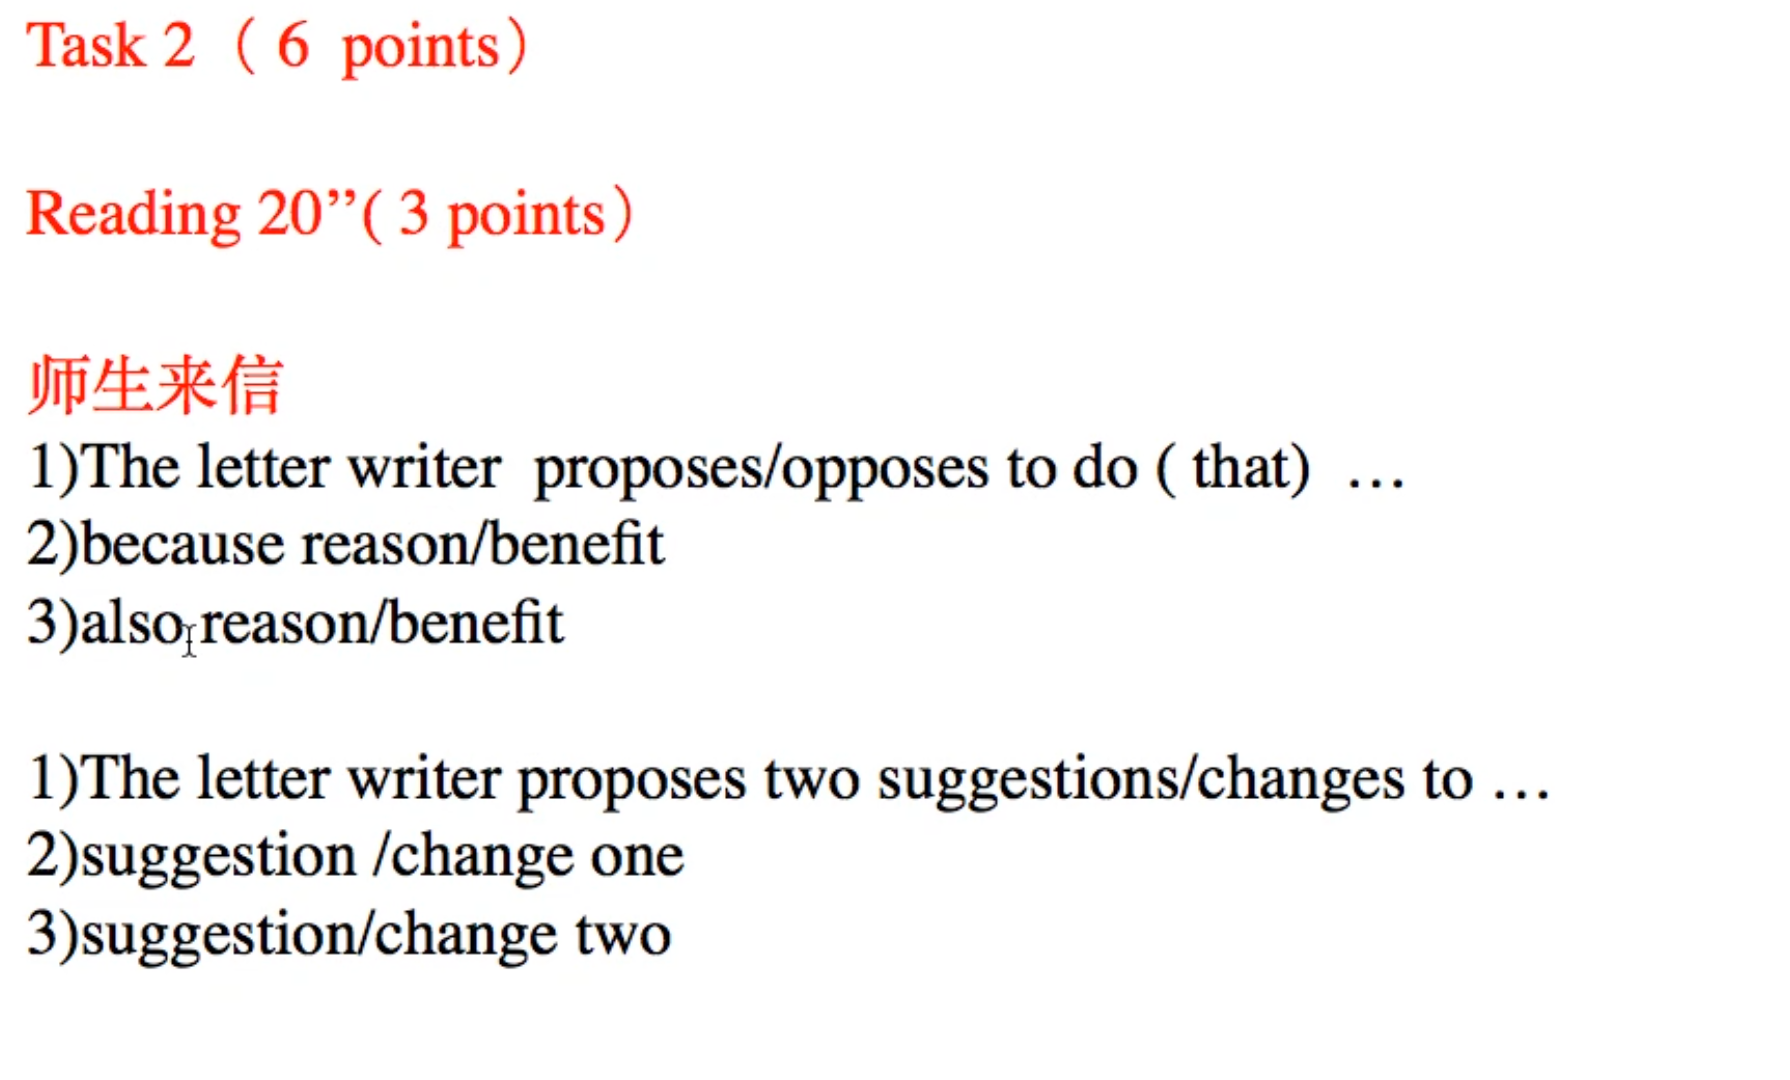
\includegraphics[width=.8\linewidth]{image1.png}
    \caption{}
  \end{figure}
  \begin{figure}[htp]
    \centering
    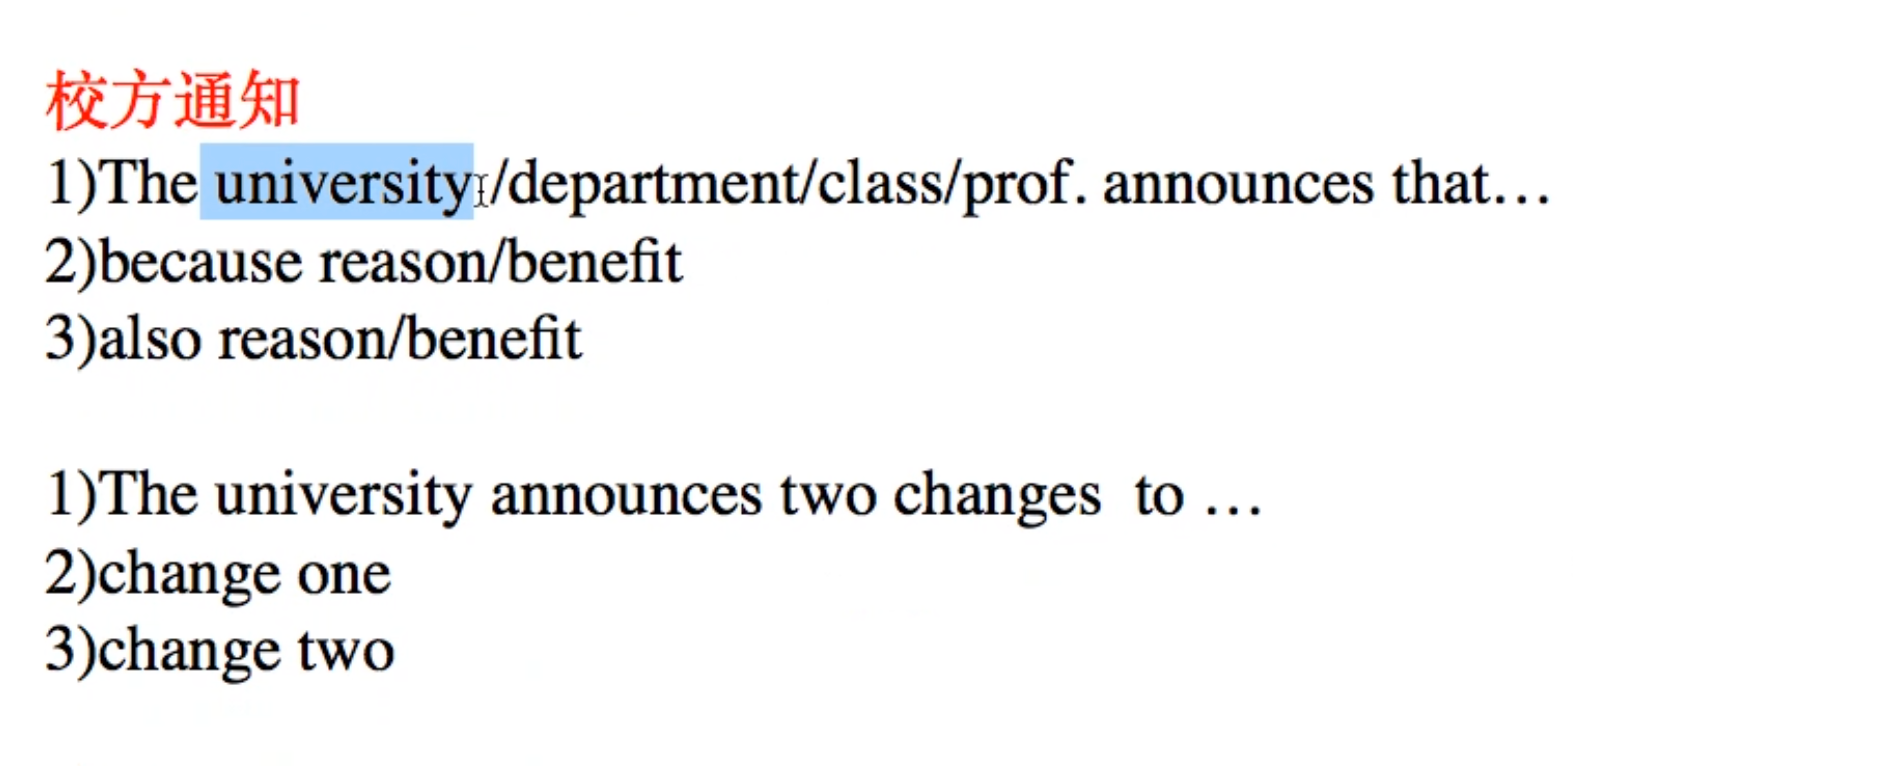
\includegraphics[width=.8\linewidth]{image2.png}
    \caption{}
  \end{figure}
  \begin{figure}[htp]
    \centering
    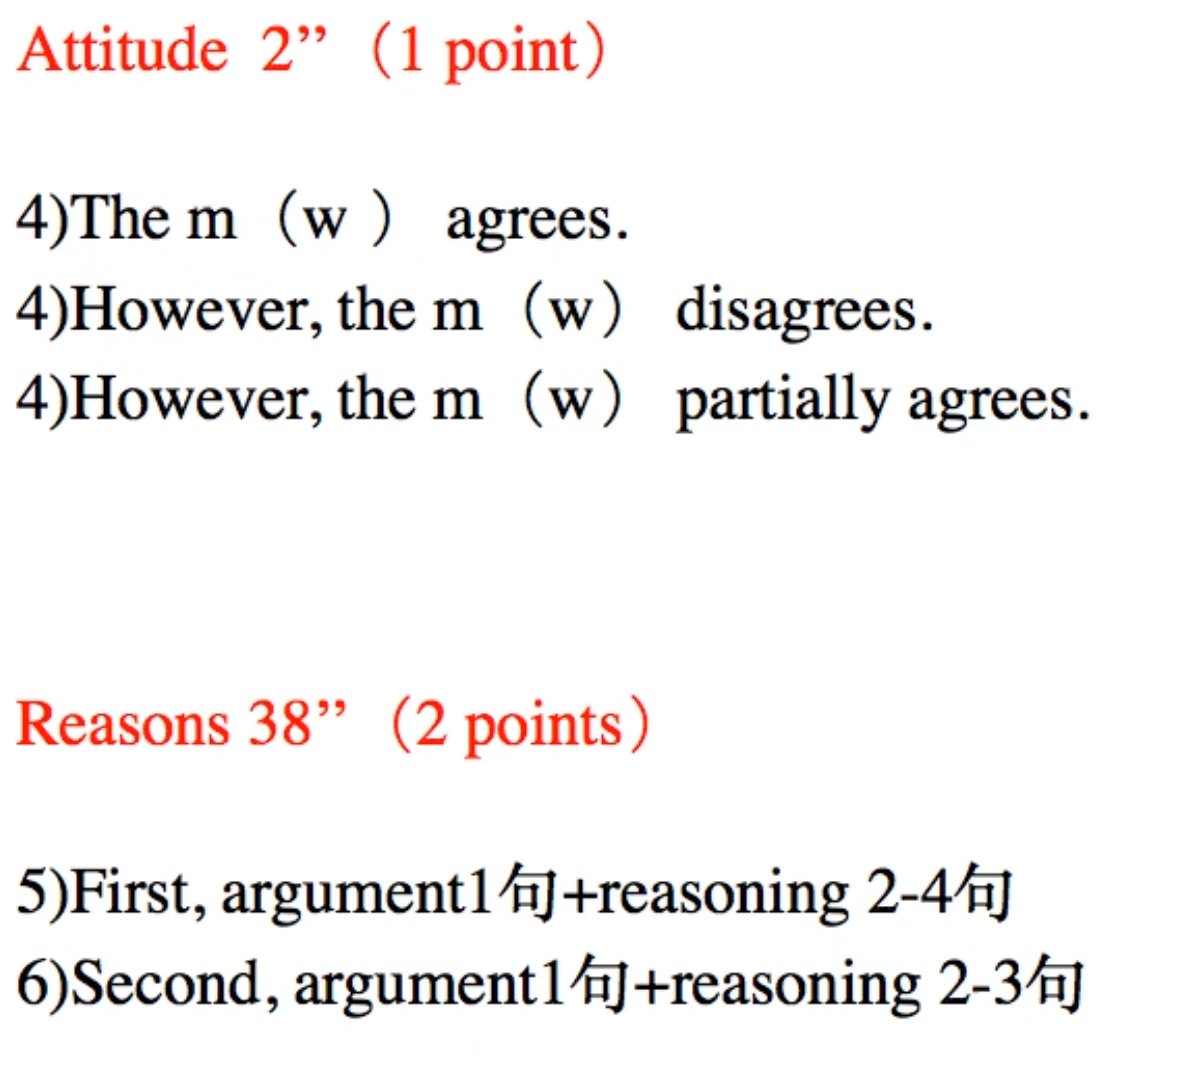
\includegraphics[width=.8\linewidth]{image3.png}
    \caption{}
  \end{figure}
  \begin{figure}[htp]
    \centering
    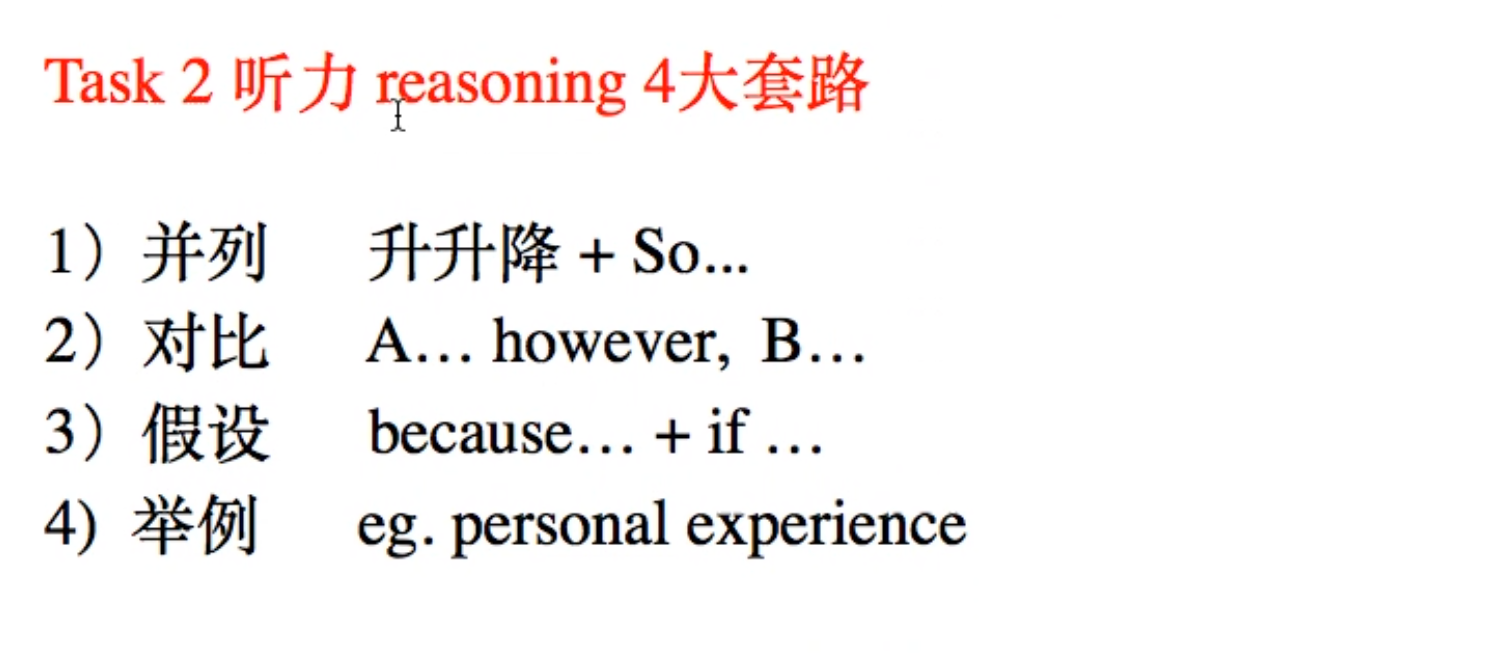
\includegraphics[width=.8\linewidth]{image4.png}
    \caption{}
  \end{figure}
\end{document}
